\documentclass[xcolor=table]{beamer}
\usetheme{uic}
\usepackage{amsfonts,amsmath,oldgerm,algorithmic,algorithm}
\usepackage[font=small,labelfont=bf]{caption} % Required for specifying captions to tables and figures
\usepackage{tcolorbox}
\tcbuselibrary{listings,skins}
\usepackage{alltt,xcolor}
\usepackage{hyperref}
\usepackage{comment}
\usepackage{amsthm}
\usepackage[spanish,es-noshorthands]{babel}
\usepackage{tikz}
\usetikzlibrary{calendar}


\lstdefinestyle{mystyle}{
language=C
}

\newtcblisting{mylisting}[2][]{
    arc=0pt, outer arc=0pt,
    listing only, 
    listing style=mystyle,
    title=#2,
    #1
}


\newcommand{\hrefcol}[2]{\textcolor{uihteal}{\href{#1}{#2}}}
\newcommand{\testcolor}[1]{\colorbox{#1}{\textcolor{#1}{test}}~\texttt{#1}}

% Please see Section 18.1 of Beamer User Guide for all the options \usefonttheme provides
\usefonttheme[onlymath]{serif}
% \usefonttheme{serif} % use this if you would like Serif font throughout (and not just for math)

\title{Fundamentos de Inteligencia Artificial}
\titlebackground{images/etsiinformatica3.jpeg}
% an asterisk will split the background:
% \titlebackground*{images/uic_seo.jpg}
\subtitle{Práctica 1. Lenguaje While}

\author{\href{mailto:jmmontes@uma.es}{José A. Montenegro}}
\date{\today}



\begin{document}

\newtheorem{mydef}{Definición}[section] % Añade [section] para que se reinicie en cada sección
\maketitle

% default is no footline, but page numbers are incredibly useful for the audience to ask questions later
\footlinecolor{uicblue}

%%%%%%%%%%%%%%%%%%%%%%%%%%%%%%%%%%%%%%%%%%%%%%%%%%%
%%%%%%%%%%%%%%%%%%%%%%%%%%%%%%%%%%%%%%%%%%%%%%%%%%%
%%%%%%%%%%%%%%%%%%%%%%%%%%%%%%%%%%%%%%%%%%%%%%%%%%%
%%%%%%%%%%%%%%%%%%%%%%%%%%%%%%%%%%%%%%%%%%%%%%%%%%%
%%%%%%%%%%%%%%%%%%%%%%%%%%%%%%%%%%%%%%%%%%%%%%%%%%%
%%%%%%%%%%%%%%%%%%%%%%%%%%%%%%%%%%%%%%%%%%%%%%%%%%%


%%%%%%%%%%%%%%%%%%%%%%%%%%%%%%%%%%%%%%%%%%%%%%%%%%%
%%%%%%%%%%%%%%%%%%%%%%%%%%%%%%%%%%%%%%%%%%%%%%%%%%%
%%%%%%%%%%%%%%%%%%%%%%%%%%%%%%%%%%%%%%%%%%%%%%%%%%%
%%%%%%%%%%%%%%%%%%%%%%%%%%%%%%%%%%%%%%%%%%%%%%%%%%%
%%%%%%%%%%%%%%%%%%%%%%%%%%%%%%%%%%%%%%%%%%%%%%%%%%%
%%%%%%%%%%%%%%%%%%%%%%%%%%%%%%%%%%%%%%%%%%%%%%%%%%%
%###########################################################################
% Contenidos
%###########################################################################
\small


%\begin{frame}{Contenido}
%\tableofcontents
%\end{frame}


%\section{Información de contacto}



%%%%%%%%%%%%%%%%%%%%%%%%%%%%%%%%
\begin{frame} \frametitle{Ejercicios} 




\begin{enumerate}
    \item Explique que computa la siguiente función WHILE-calculable: \\

(2,2,$X_2 :=X_2+1$; $while X_1 \neq$ =0 do $X_1$:=$X_1$-1; $X_2$ :=$X_2$-1 od; $X_1$ :=$X_2$)

\item El programa  WHILE más simple sin argumentos que computa la función   \textit{diverge}.
 
\item Implementa un programa WHILE que computa la suma de tres valores.


\end{enumerate}


\end{frame} 


%%%%%%%%%%%%%%%%%%%%%%%%%%%%%%%%
%%%%%%%%%%%%%%%%%%%%%%%%%%%%%%%%


%%%%%%%%%%%%%%%%%%%%%%%%%%%%%%%%
\begin{frame} \frametitle{Ejercicio 1}  \footnotesize  


\begin{enumerate}
\item Abre el archivo ``ExampleWHILE.txt''.

 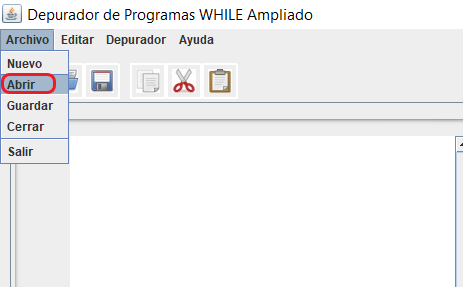
\includegraphics[scale=0.3]{images/p3r1}
 
\item Cargamos el programa en la flecha verde que está situada en el panel de la derecha.

 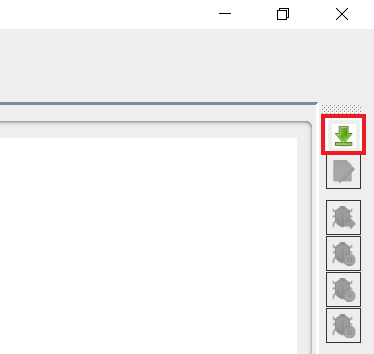
\includegraphics[scale=0.3]{images/p3r2}

 \end{enumerate}
\end{frame} 

%%%%%%%%%%%%%%%%%%%%%%%%%%%%%%%%
\begin{frame} \frametitle{Ejercicio 1} \footnotesize  

\begin{enumerate}
\setcounter{enumi}{2}

\item A continuación aparecerá un mensaje que nos pedirá el valor de las variables, introducimos los valores X1=5 y X2=4.

 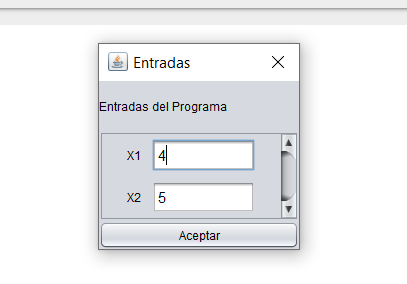
\includegraphics[scale=0.3]{images/p3r3}

 
\item Podemos ejecutar el programa directamente con el icono del 'bicho' o  paso a paso. En la consola irá mostrándose las configuraciones de la ejecución.

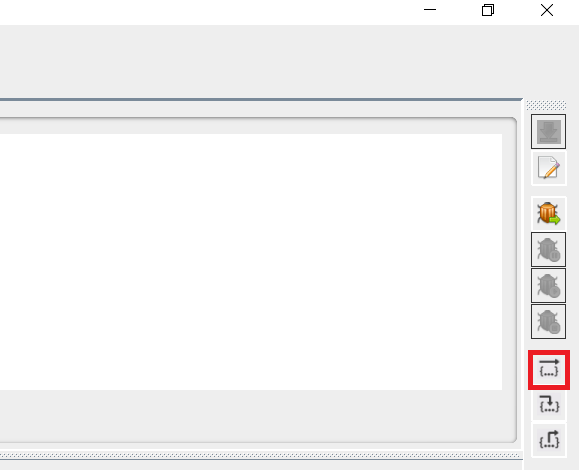
\includegraphics[scale=0.2]{images/p3r4}
\end{enumerate}

\end{frame} 

%%%%%%%%%%%%%%%%%%%%%%%%%%%%%%%%
\begin{frame} \frametitle{Ejercicio 1} \footnotesize  

\begin{enumerate}
\setcounter{enumi}{4}

\item ¿Cuál es la configuración inicial del programa? ¿Y la final?

La primera configuración es (1,5,4) y la última es: (7,0,0).

\item Calcula $SIG_Q (1,3,3), CAL_Q (3,3,6), T_Q (3,3), F_Q (3,3)$.

\begin{itemize}
        \item $SIG_Q (1,3,3) = (2,3,4)$
        \item $CAL_Q (3,3,6) = (3,2,3)$
        \item $T_Q (3,3) = 15$
        \item $F_Q (3,3) = 1$
    \end{itemize}
    
\item Calcula $F_Q (4,5), F_Q (5,3), F_Q (2,1), F_Q (3,7)$. ¿Qué computa esta función?

\begin{itemize}
        \item $F_Q (4,5) = 2$
        \item $F_Q (5,3) = 0$
        \item $F_Q (2,1) = 0$
        \item $F_Q (3,7) = 5$
    \end{itemize}
\end{enumerate}
\end{frame} 

%%%%%%%%%%%%%%%%%%%%%%%%%%%%%%%%
\begin{frame}  \frametitle{Ejercicio 1}

\begin{itemize}
    \item La función que computa este programa WHILE es: $f(x,y)=y-x+1$.
     
    \item Si igualamos esta función a cero, podemos definir un predicado lógico que define $f$, por lo que cuando $f>0$ (verdadero) o $f=0$ (falso).
 
    \item $$f(x,y)>0 \iff y-x+1 >0 \iff y >x-1 \iff y \geq x$$ 
    \item Por tanto, podemos definir que el predicado lógico que define es: ``Sea $y$ mayor o igual que $x$''.
\end{itemize}
\end{frame} 

%%%%%%%%%%%%%%%%%%%%%%%%%%%%%%%%
\begin{frame}  \frametitle{Ejercicio 1}

\begin{enumerate}
\setcounter{enumi}{5}
    \item \textbf{$CAL_Q$(3,3,6) = (3,2,3)} \\
    $CAL_Q$(3,3,6)= \\
$SIG_Q$($CAL_Q$(3,3,5))=$SIG_Q$($SIG_Q$($CAL_Q$(3,3,4)))= \\
$SIG_Q$($SIG_Q$($SIG_Q$($CAL_Q$(3,3,3))))= $SIG_Q$($SIG_Q$($SIG_Q$($SIG_Q$($CAL_Q$(3,3,2)))))=\\ $SIG_Q$($SIG_Q$($SIG_Q$($SIG_Q$($SIG_Q$($CAL_Q$(3,3,1))))))= $SIG_Q$($SIG_Q$($SIG_Q$($SIG_Q$($SIG_Q$($SIG_Q$($CAL_Q$(3,3,0))))))= $SIG_Q$($SIG_Q$($SIG_Q$($SIG_Q$($SIG_Q$($SIG_Q$(1,3,3))))))= $SIG_Q$($SIG_Q$($SIG_Q$($SIG_Q$($SIG_Q$(2,3,4)))))= $SIG_Q$($SIG_Q$($SIG_Q$($SIG_Q$(3,3,4))))=$SIG_Q$($SIG_Q$($SIG_Q$(4,2,4))))= \\
$SIG_Q$($SIG_Q$(5,2,3))))=$SIG_Q$(2,2,3)=(3,2,3)

\end{enumerate}

\end{frame} 

%%%%%%%%%%%%%%%%%%%%%%%%%%%%%%%%
\begin{frame}  \frametitle{Ejercicio 1}

\begin{enumerate}
\setcounter{enumi}{5}
    \item 
    \begin{itemize}
    \item \textbf{$T_Q$(3,3)=15($\vdash$)} \\
(1,3,3) $\vdash$(2,3,4) $\vdash$(3,3,4) $\vdash$(4,2,4) $\vdash$ (5,2,3)\\ 
$\vdash$ (2,2,3) $\vdash$(3,2,3) $\vdash$(4,1,3) $\vdash$(5,1,2)\\ 
$\vdash$ (2,1,2) $\vdash$(3,1,2) $\vdash$(4,0,2) $\vdash$(5,0,1)\\ 
$\vdash$ (2,0,1) $\vdash$ (6,0,1) $\vdash$ (7,1,1) \\
  \item \textbf{$F_Q$(3,3)}= $\pi^3_2$ (7,1,1) = 1

    \end{itemize}
  \item \textbf{$F_Q$ (4,5)= $\pi^3_2$ (7,2,2) = 2}\\ 
  (1,4,5) $\vdash$(2,4,6) $\vdash$(3,4,6) $\vdash$(4,3,6) $\vdash$(5,3,5) $\vdash$(2,3,5) $\vdash$(3,3,5) \\
  $\vdash$(4,2,5) $\vdash$(5,2,4) $\vdash$(2,2,4) $\vdash$(3,2,4) $\vdash$(4,1,4) $\vdash$(5,1,3) $\vdash$(2,1,3) \\
  $\vdash$(3,1,3) $\vdash$(4,0,3) $\vdash$(5,0,2) $\vdash$(2,0,2)$\vdash$(5,0,2) $\vdash$(6,2,2) $\vdash$(7,2,2) 

\end{enumerate}

\end{frame} 

%%%%%%%%%%%%%%%%%%%%%%%%%%%%%%%%
\begin{frame}  \frametitle{Ejercicio 1}

\begin{enumerate}
\setcounter{enumi}{6}
    \item 
    
    
    \begin{itemize}
    \item \textbf{$F_Q$(5,3)= $\pi^3_2$ (7,0,0)= 0} \\
    (1,5,3) $\vdash$ (2,5,4) $\vdash$ (3,5,4) $\vdash$ (4,4,4) $\vdash$ (5,4,3) $\vdash$ (2,4,3) $\vdash$ (3,4,3) \\
    $\vdash$ (4,3,4) $\vdash$ (5,3,3) $\vdash$ (2,3,3) $\vdash$ (3,3,3) $\vdash$ (4,2,3) $\vdash$ (5,2,2) $\vdash$ (2,2,2) \\
    $\vdash$ (3,2,2) $\vdash$ (4,1,2) $\vdash$ (5,1,1) $\vdash$ (2,1,1) $\vdash$ (3,1,1) $\vdash$ (4,0,1) $\vdash$ (5,0,0) \\
    $\vdash$ (2,0,0) $\vdash$ (6,0,0) $\vdash$ (7,0,0)

    \item \textbf{$F_Q$ (2,1)= $\pi^3_2$ (7,0,0)= 0} \\
    (1,2,1) $\vdash$ (2,2,2) $\vdash$ (3,2,2) $\vdash$ (4,1,2) $\vdash$ (5,1,1) $\vdash$ (2,1,1) $\vdash$ (3,1,1) \\
    $\vdash$ (4,0,1) $\vdash$ (5,0,0) $\vdash$ (2,0,0) $\vdash$ (6,0,0) $\vdash$ (7,0,0) 

    \item \textbf{$F_Q$ (3,7)= $\pi^3_2$ (7,5,5)= 5} \\
    (1,3,7) $\vdash$ (2,3,8) $\vdash$ (3,3,8) $\vdash$ (4,2,8) $\vdash$ (5,2,7) $\vdash$ (2,2,7) $\vdash$ (3,2,7)  \\ 
    $\vdash$ (4,1,7) $\vdash$ (5,1,6) $\vdash$ (2,1,6) $\vdash$ (3,1,6) $\vdash$ (4,0,6) $\vdash$ (5,0,5) $\vdash$ (2,0,5) \\ 
    $\vdash$ (6,5,5) $\vdash$ (7,5,5)

    \end{itemize}
 





\end{enumerate}

\end{frame} 

%%%%%%%%%%%%%%%%%%%%%%%%%%%%%%%%
\begin{frame} \frametitle{Ejercicio 2} \small  


\begin{columns}

\begin{column}{0.43\textwidth}
Q = (0,1,s) \\

s: \\
$X_1$ := $X_1$+1; \\
while $X_1 \neq 0 $ do \\
\hspace{0.3cm}$X_1$ := $X_1$+1 \\
od \\


\end{column}

\begin{column}{0.43\textwidth}

Q = (0,2,s) \\

s: \\
$X_2$ := $X_1$+1; \\
while $X_2 \neq 0 $ do \\
\hspace{0.3cm}$X_1$ := 0 \\
od \\
\end{column}

\end{columns}

\end{frame} 


%%%%%%%%%%%%%%%%%%%%%%%%%%%%%%%%
\begin{frame} \frametitle{Ejercicio 3} \small  


\begin{columns}

\begin{column}{0.43\textwidth}
Q = (3,3,s) \\

s: \\

while $X_2 \neq 0 $ do \\
\hspace{0.3cm}$X_1$ := $X_1$+1; \\
\hspace{0.3cm}$X_2$ := $X_2$-1 \\
od; \\

while $X_3 \neq 0 $do\\ 
\hspace{0.3cm}$X_1$ := $X_1$+1; \\
\hspace{0.3cm}$X_3$ := $X_3$-1 \\
od\\

\end{column}

\begin{column}{0.43\textwidth}


    Q = (3,4,s)\\
    s:\\
    
    $X_4:=X_1;$\\
    while $X_2 \neq 0 $ do\\
    \hspace{0.3cm}$X_4$:=$X_4$ + 1;\\
    \hspace{0.3cm}$X_2$:=$X_2$ - 1\\
    od;\\
    
    while $X_3 \neq 0 $ do\\
    \hspace{0.3cm}$X_4$:=$X_4$ + 1;\\
    \hspace{0.3cm}$X_3$:=$X_3$ - 1\\
    od\\
    $X_1$:=$X_4$\\
\end{column}

\end{columns}

\end{frame} 





%%%%%%%%%%%%%%%%%%%%%

% \begin{frame}  \small
 
  %\begin{figure}[!hbtp]
%\begin{center}
%	\includegraphics[scale=0.3]{imagenes/system-architecture.jpg} 
%		  \caption{Arquitectura del Sistema}
%\end{center}
%\end{figure}
%\end{frame}









%%%%%%%%%%%%%%%%%%%%%%%%%%%%%%%%
%\begin{frame}  \small  
%\end{frame} 


%%%%%%%%%%%%%%%%%%%%%%%%%%%%%%%%
%\begin{frame}  \small  
%\end{frame} 


%%%%%%%%%%%%%%%%%%%%%%%%%%%%%%%%
%\begin{frame}  \small  
%\end{frame} 

%%%%%%%%%%%%%%%%%%%%%%%%%%%%%%%%%%%%%%%%%%%%%%%%%%%
%%%%%%%%%%%%%%%%%%%%%%%%%%%%%%%%%%%%%%%%%%%%%%%%%%%
%%%%%%%%%%%%%%%%%%%%%%%%%%%%%%%%%%%%%%%%%%%%%%%%%%%

%%\begin{chapter}[images/etsiinformatica4.png]{uicblue}{Introducción}
%\end{chapter}

%%%%%%%%%%%%%%%%%%%%%%%%%%%%%%%%%%%%%%%%%%%%%%%%%%%
%%%%%%%%%%%%%%%%%%%%%%%%%%%%%%%%%%%%%%%%%%%%%%%%%%%


%%%%%%%%%%%%%%%%%%%%%%%%%%%%%%%%%%%%%%%%%%%%%%%%%%%
%%%%%%%%%%%%%%%%%%%%%%%%%%%%%%%%%%%%%%%%%%%%%%%%%%%
%%%%%%%%%%%%%%%%%%%%%%%%%%%%%%%%%%%%%%%%%%%%%%%%%%%
%%%%%%%%%%%%%%%%%%%%%%%%%%%%%%%%%%%%%%%%%%%%%%%%%%%



\backmatter


\end{document}